\documentclass[a4paper,12pt]{article}
\usepackage{cite}
\usepackage[a4paper, margin=1.5in]{geometry}
\usepackage{amsmath,amssymb,amsfonts,amsthm}
\usepackage{algorithmic}
\usepackage{graphicx}
\usepackage{textcomp}
\usepackage{xcolor}
\usepackage{txfonts}
\usepackage{listings}
\usepackage{enumitem}
\usepackage{graphicx}
\usepackage{mathtools}
\usepackage{gensymb}
\usepackage{comment}
\usepackage[siunitx, american]{circuitikz}
\usepackage[breaklinks=true]{hyperref}
\usepackage{tkz-euclide} 
\usepackage{listings}
\usepackage{gvv}        
\usepackage{float}
\usepackage{amsmath}
%\def\inputGnumericTable{}                                 
\usepackage[latin1]{inputenc}     
\usepackage{xparse}
\usepackage{color}                                            
\usepackage{array}                                            
\usepackage{longtable}                                       
\usepackage{calc}                                             
\usepackage{multirow}
\usepackage{multicol}
\usepackage{hhline}                                           
\usepackage{ifthen}     
\usepackage{placeins}
\usepackage{lscape}
\usepackage{tabularx}
\usepackage{array}
\usepackage{float}
\usepackage{listings}
\usepackage{xcolor}
\usepackage{booktabs}
\usepackage{caption}
\usepackage{tikz}
\usetikzlibrary{automata, arrows.meta}

\lstset{
  language=Python,
  basicstyle=\ttfamily\small,
  keywordstyle=\color{orange}\bfseries,
  stringstyle=\color{green!60!black},
  commentstyle=\color{gray},
  identifierstyle=\color{blue!70!black},
  numbers=left,
  numberstyle=\tiny\color{gray},
  frame=single,
  breaklines=true,
  showstringspaces=false,
  xleftmargin=0.2cm,
  xrightmargin=0cm,
  framexleftmargin=0.2cm,
  backgroundcolor=\color{gray!5}
}


\newtheorem{theorem}{Theorem}[section]
\newtheorem{problem}{Problem}
\newtheorem{proposition}{Proposition}[section]
\newtheorem{lemma}{Lemma}[section]
\newtheorem{corollary}[theorem]{Corollary}
\newtheorem{example}{Example}[section]
\newtheorem{definition}[problem]{Definition}
\newcommand{\BEQA}{\begin{eqnarray}}
\newcommand{\EEQA}{\end{eqnarray}}
\theoremstyle{remark}
\renewcommand{\thefigure}{\arabic{figure}}

\begin{document}
\title{1.1.63}
\author{ee25Btech11063 (Yalamati Vejith) }
\maketitle
\renewcommand{\thefigure}{\theenumi}
\renewcommand{\thetable}{\theenumi}
\textbf{Question}\\
The natural frequency of the system shown below is \hspace{3cm}(ME 2007)
\begin{figure}[H]
    \centering
    
\includegraphics[width=0.9\columnwidth]{figs/01.png}
    \label{fig:placeholder}
\end{figure}
\begin{enumerate}[label=\alph*)]
\begin{multicols}{4}
     \item $\sqrt{\frac{k}{2m}}$
      \item $\sqrt{\frac{k}{m}}$
      \item $\sqrt{\frac{2k}{m}}$
      \item $\sqrt{\frac{3k}{m}}$
\end{multicols}
   \end{enumerate}
   \textbf{Solution :}\\
Two springs of stiffness $k/2$ are connected in parallel, and this combination is in series with a spring of stiffness $k$, attached to a mass $m$.
\\ \\
\textbf{Parallel Combination :} 

Springs are in parallel when they have the same displacement. The equivalent stiffness is:
\begin{align}
    k_{\text{parallel}} = k_1 + k_2
\end{align}


Here,
\begin{align}
    k_{\text{parallel}} = \frac{k}{2} + \frac{k}{2} = k 
\end{align}


\textbf{Series Combination :} 
Springs are in series when they experience the same force. The equivalent stiffness is:
\begin{align}
    \frac{1}{k_{\text{eq}}} = \frac{1}{k_1} + \frac{1}{k_2}
\end{align}


Thus,
\begin{align}
    \frac{1}{k_{\text{eq}}} = \frac{1}{k} + \frac{1}{k} = \frac{2}{k}
\end{align}

\begin{align}
    k_{\text{eq}} = \frac{k}{2}
\end{align}


\bigskip

\textbf{Natural Frequency :}

The natural frequency is given by:
\begin{align}
    \omega_n = \sqrt{\frac{k_{\text{eq}}}{m}}
\end{align}


Substituting,
\begin{align}
  \implies  \omega_n = \sqrt{\frac{k}{2m}}
\end{align}
\textbf{Python Plot :}
\begin{figure}[H]
    \centering
    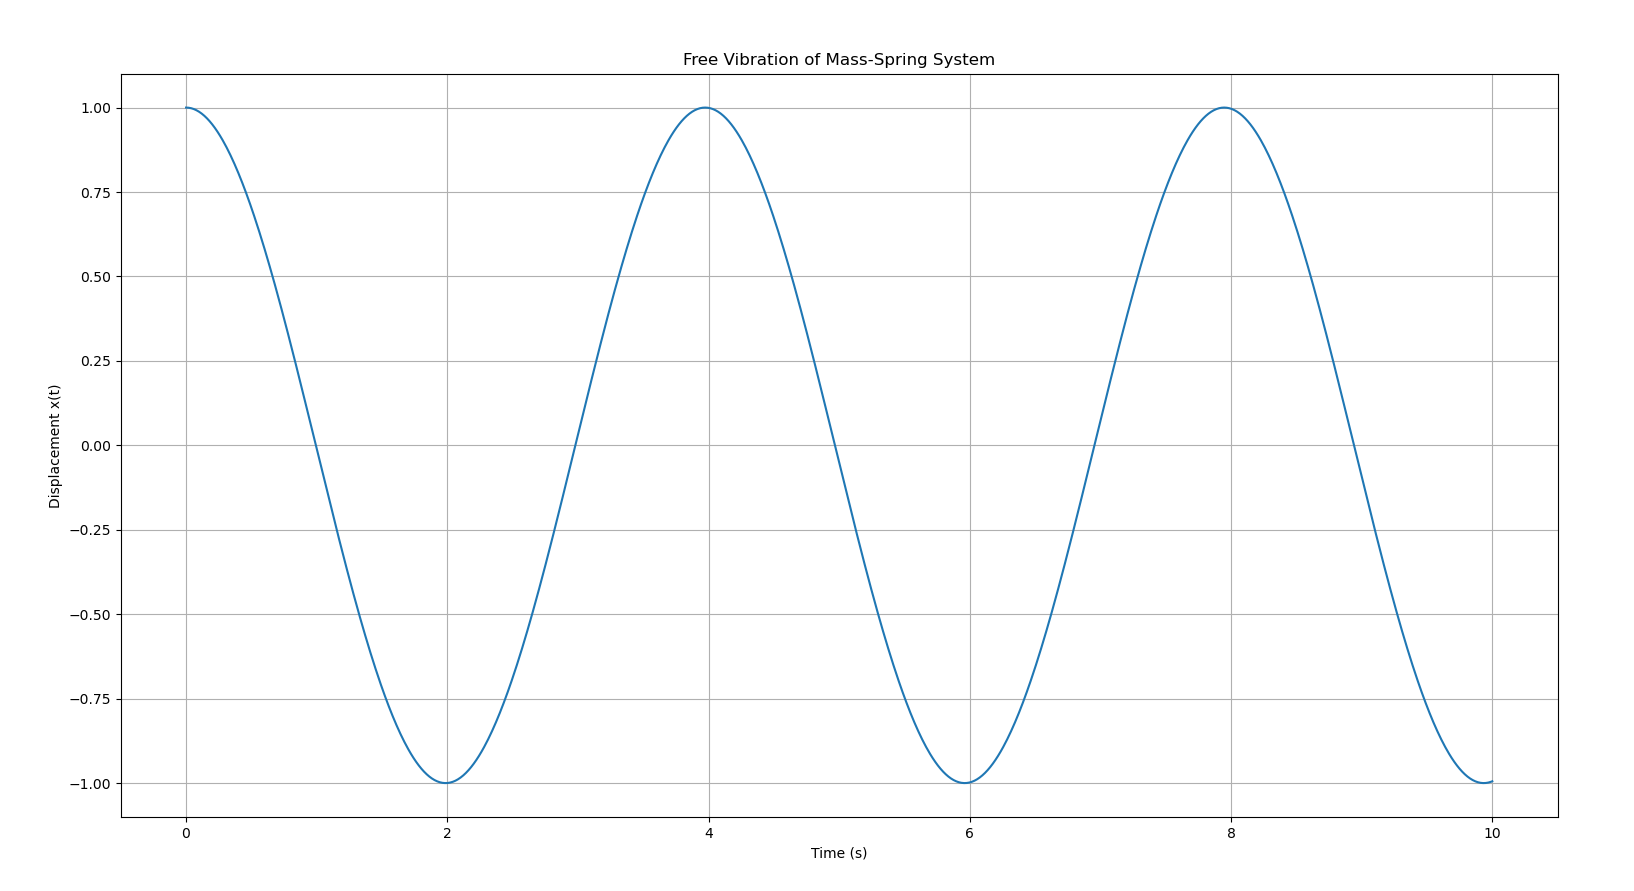
\includegraphics[width=1.3\columnwidth]{figs/02.png}
    \label{fig:placeholder}
\end{figure}
\end{document}
